\section{Local Model Agnostic}

\subsection{ICE - Individual Conditional Expectation }
\textit{How a samples prediction changes, when all but one features are fixed and then the remaining feature
	gets replace by values from a grid}
\begin{enumerate}
	\item Keep all but one features fixed.
	\item Replace remaining feature with values from a grid of reasonable values for that feature.
	\item Record how the prediction changes while varying that feature.
	\item Plot the change. With $y$ axis, the predicted value, $x$ axis the values of the feature.
\end{enumerate}

\begin{itemize}
	\item Shows how the instances prediction changes when a feature changes.
	\item Visualizes the dependence of the prediction on a feature for each instance separately
\end{itemize}
\paragraph{ICE-Plot}
\begin{figure}[H]
	\begin{center}
		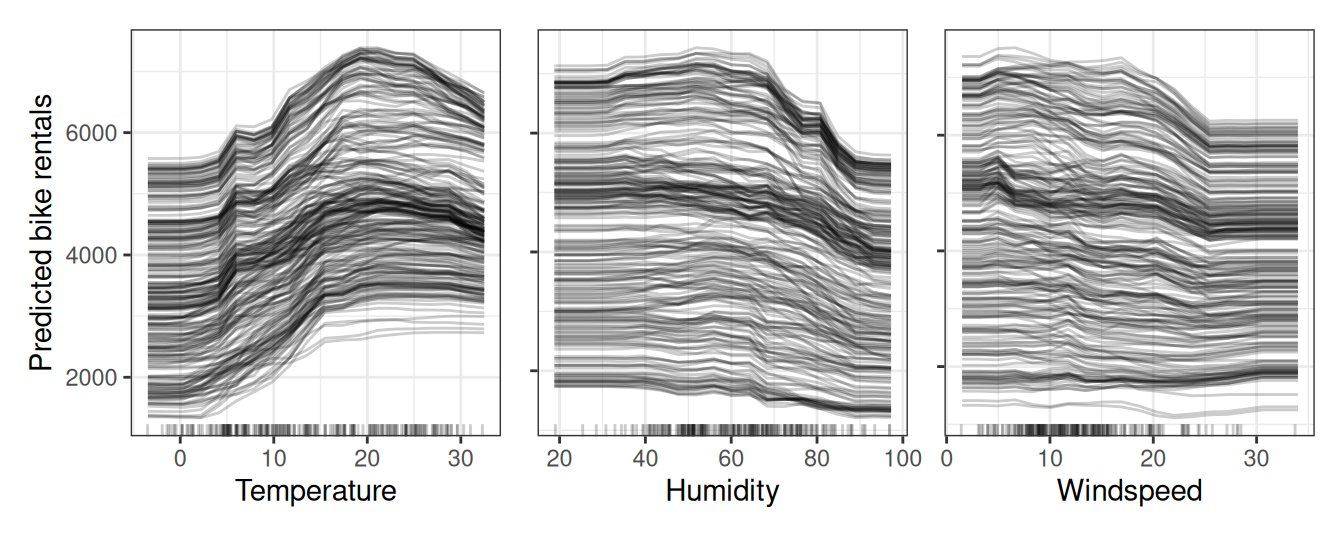
\includegraphics[width=0.95\linewidth]{images/fig-ice-bike-1.png}
	\end{center}
	\caption{ICE-Plot}\label{fig:ICE-Plot}
\end{figure}
\paragraph{Centered ICE-Plot}
Since it is hard to see sometimes, if the individual curves are different from one another, they are usually centered.
To center the curves subtract the intercept of each curve. They start at different intercepts, because the data points are different (duh).
\begin{figure}[H]
	\begin{center}
		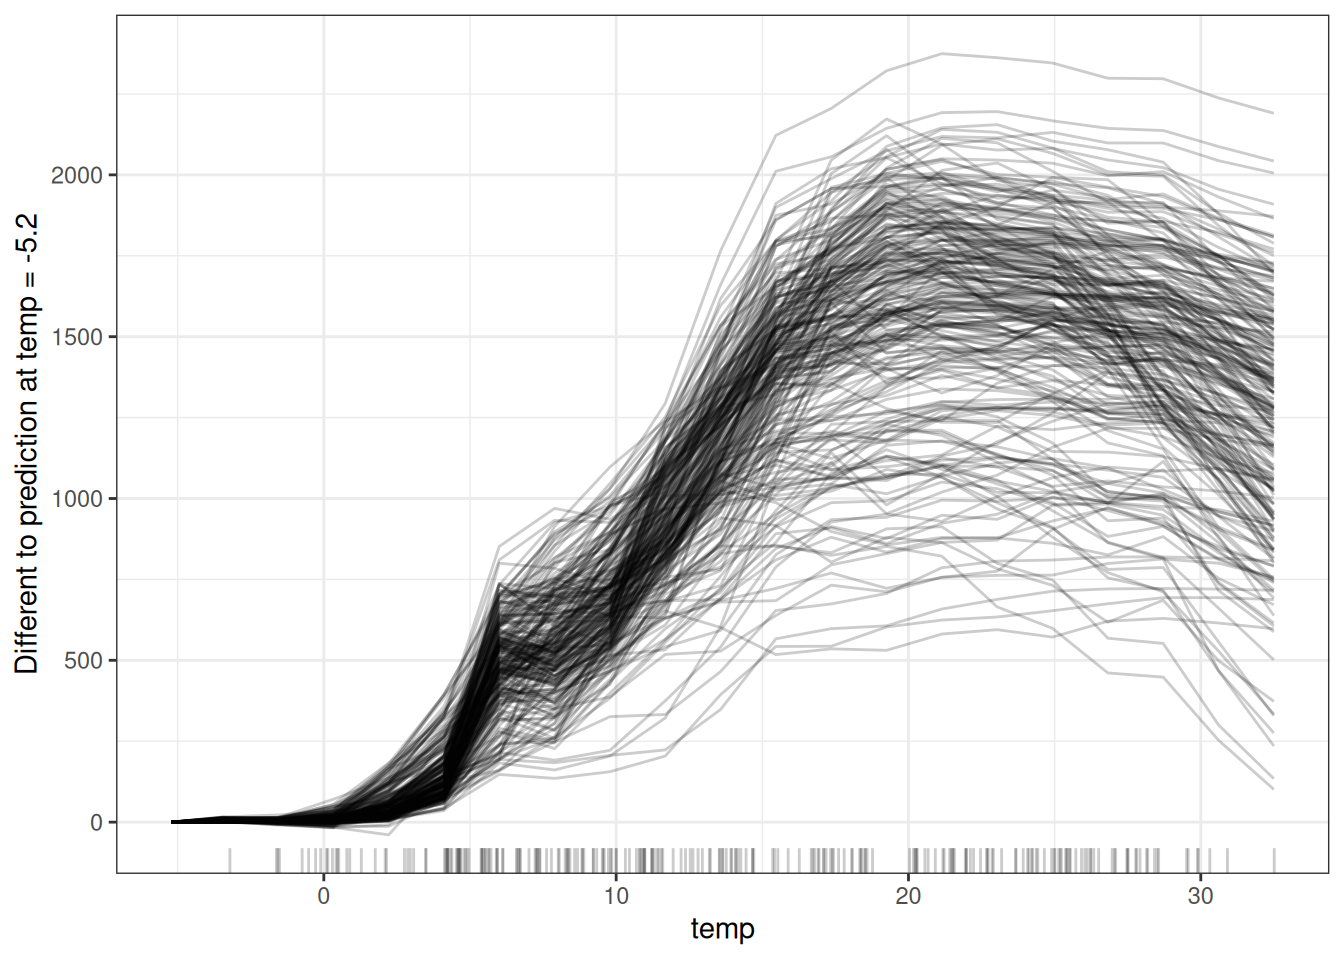
\includegraphics[width=0.45\linewidth]{images/ice-bike-centered-1.png}
	\end{center}
	\caption{Centered-ICE Plot}\label{fig:ICE-Centerd}
\end{figure}
Connected to ICE; A Partial Dependence Plots is just the average of all ICE curves.
Often, when the  ICE curves are too crowded,

\paragraph{Derivative ICE-Plot}
Instead of the raw data, plots the derivative of each ICE-curve.
\begin{itemize}
	\item Show where and how strongly predictions change
	\item Derivatives tell in which direction change occurs.
	\item Makes it easy to spot in which ranges the predictions change.
	\item Spot non-linearity (linear relationship is flat line)
\end{itemize}


\subsection{LIME - Local Interpretable Model-Agnostic Explanations}
\textit{Explain model predictions by using local surrogate models.}
\begin{figure}[H]
	\begin{center}
		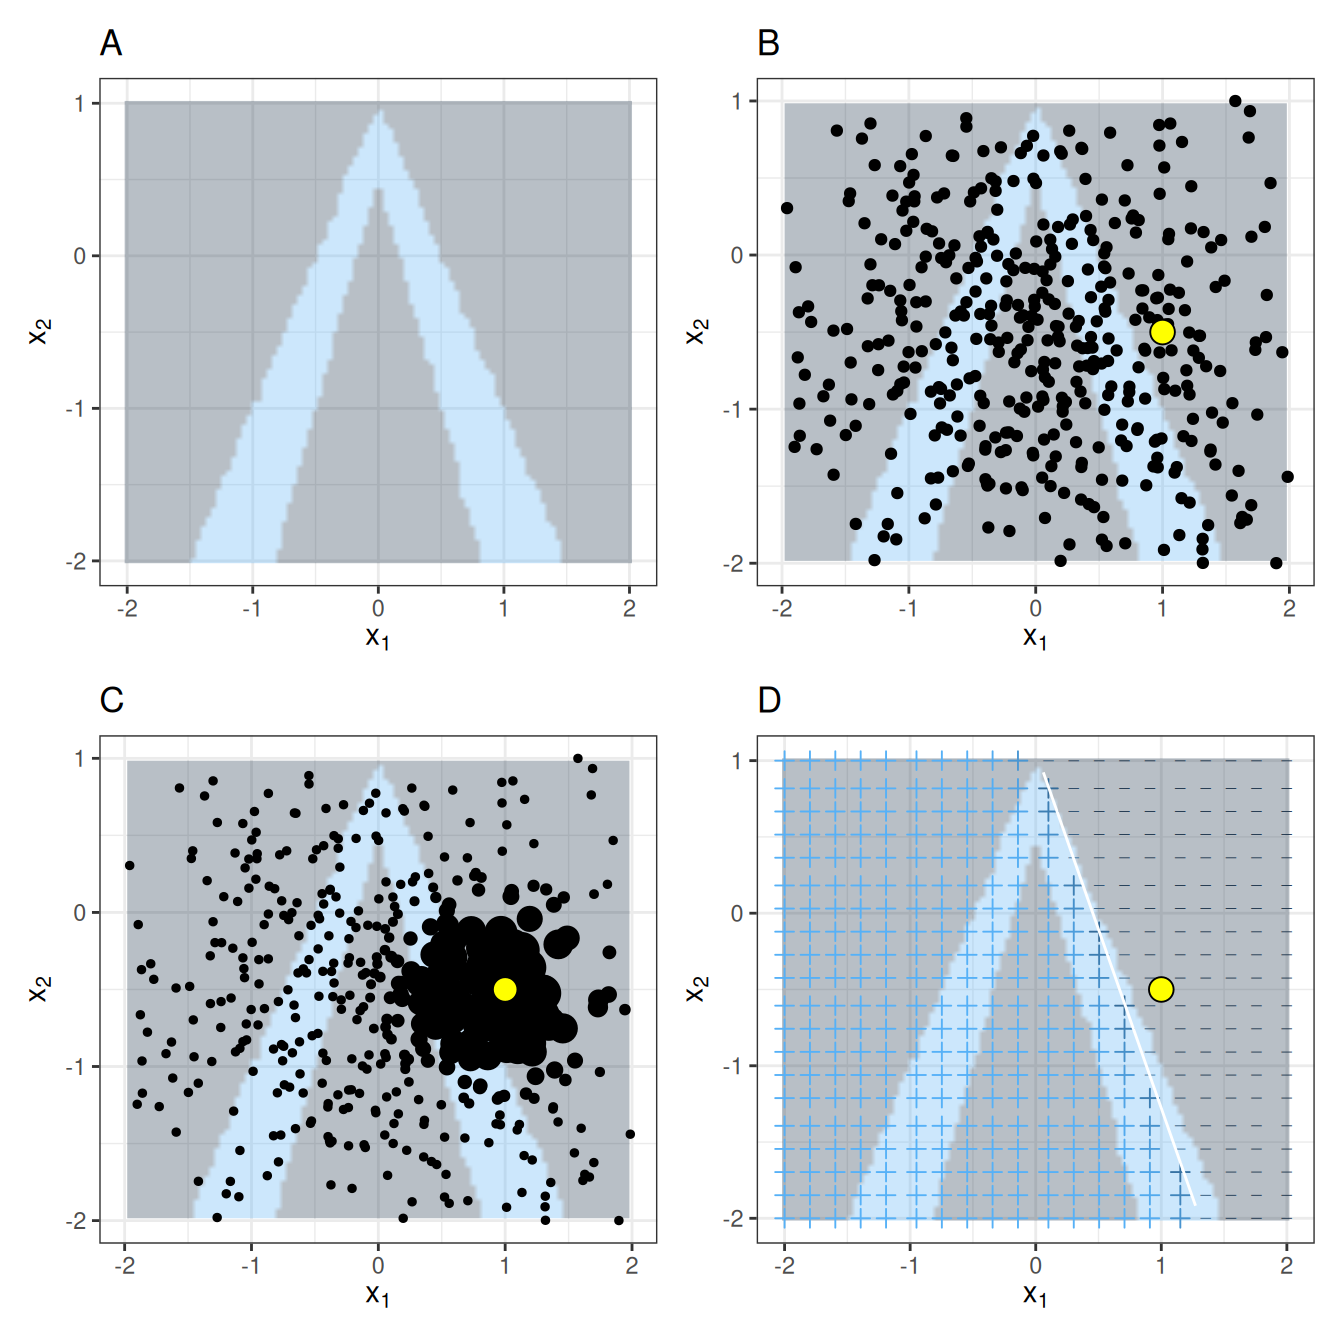
\includegraphics[width=0.9\linewidth]{images/fig-lime-fitting-1.png}
	\end{center}
	\caption{LIME explanations  $a \to b \to c \to d$ \\ Background is the black-box models predictions}\label{fig:Lime-Model-Fitting}
\end{figure}

\paragraph{LIME}
\begin{equation}
	\text{explanation}(x) = \argmin{g \in G} L \lr{\hat f, g, \pi_x} + \Omega(g)
	\label{eq:LIME-Explanation}
\end{equation}
where
\begin{itemize}
	\item explanation is the model g, that minimizes the Loss.
	\item Loss measures how close the explanation model $g$ is to the original $hat f $.
	\item $\pi_x$: Defines how large the neighborhood around instance x is, that we consider for the explanations.
	      This is done by weighting the points in the dataset using an exponential kernel.
	\item $\Omega(g)$: Complexity of the model. Has to be set by the user. LIME only optimizes the loss part.
\end{itemize}

\paragraph{LIME Algorithm}
\begin{enumerate}
	\item Choose instance to explain.
	\item Generate a new dataset by perturbing the instance (generate variations of it to generate similar instances).
	      \begin{itemize}
		      \item Tabular: Get $\mu, \sigma$ from the dataset (requires a few samples) and then swap the instances features with values drawn from the normal distribution.
		            Maybe its also sampled straight from the datasets mass center.
		      \item Images: Replace super-pixels (groups of connected pixel with similar colors) with a different color.
		      \item Text: Mask out some words.
	      \end{itemize}
	\item Make prediction for the perturbed dataset using the black-box model
	\item Fit the interpretable model (e.g. Linear Regression) using Equation \ref{eq:LIME-Explanation}.
	      Points close to the to be explained instance are weighted more strongly in the loss function (by the exponential kernel).
\end{enumerate}

\paragraph{Notes}
\begin{itemize}
	\item Sensitive to kernel with choice.
	\item Neighborhood definition is pretty arbitrary.
	\item Sampling features ignores correlations
\end{itemize}


\subsection{Shapley values \& SHAP}
\subsubsection{Shapley values}
\textit{Goal: Fairly attribute the difference between the average and a specific prediction to all input features.}

\paragraph{In Theory}
\begin{equation}
	\phi_j(val)=\sum_{S\subseteq\{1,\ldots,p\} \setminus \{j\}}\underbrace{\frac{|S|!\left(p-|S|-1\right)!}{p!}}_{\text{weight}} \underbrace{\left(val\left(S\cup\{j\}\right)-val(S)\right)}_{\text{Marginal contribution of $j$}}
	\label{eq:Shapley-Values}
\end{equation}
$\phi_j$, the Shapley value is the average marginal contribution of feature $j$ across all possible feature coalitions that $j$ can join.

\begin{itemize}
	\item $S$: Subset of features that does not include $j$
	\item $val_x(S)$: Prediction value using only features in $S$ (from the instance that we want to explain.)
	\item $val_x(S \setminus{j})$: Prediction value using features in $S$ and $j$
	\item $\frac{|S|!\left(p-|S|-1\right)!}{p!}$: Probability that $j$ can make that contribution. E.g. Number of ways, that $j$ can join a coalition of three other features.
\end{itemize}

The $val_\textbf{x}(S)$ is the predicted outcome of the model minus the average prediction using the defined features ($S$).
\begin{equation}
	val_{\mathbf{x}}(S)=\int\hat{f}(x_{1},\ldots,x_{p})d\mathbb{P}_{X_C}-\mathbb{E}[\hat{f}(\mathbf{X})]
	\label{eq:shap-val-function}
\end{equation}
This essentially tells us to integrate over the probability distribution of the features not in the coalition $X_C$ and get the average prediction.

\begin{equation}
	\sum_{j=1}^{p}\phi_j(\hat{f}) = \hat{f}(\mathbf{x})-\mathbb{E}[\hat{f}(\mathbf{X})]
	\label{eq:sumofshapley}
\end{equation}
The sum of Shapley values fully explains the difference from the mean prediction.

\paragraph{In Practice}
\begin{itemize}
	\item Because in ML Models we need the same amount of input features for all predictions, we can't just leave them out.
	\item All possible sets of features have to be evaluated. This quickly becomes computationally intractable for more than a few features.
\end{itemize}
Approximation using Monte-Carlo sampling
\begin{equation}
	\hat{\phi}_{j} = \frac{1}{M}\sum_{m=1}^M\left(\hat{f}(\mathbf{x}^{(m)}_{+j}) - \hat{f}(\mathbf{x}^{(m)}_{-j})\right)
	\label{eq:mc-shapley}
\end{equation}
\begin{enumerate}
	\item Replace random features in $x$ with features from a randomly sampled data point $z$
	\item Make one prediction for $x_{+j}$, where $j$ is taken from $x$ and one with $x_{-j}$ where $j$ is from $z$.
	      \\ $\to$ Marginal contribution of $j$
	\item Compare predictions
	\item Repeat $M$ times and take the mean difference as the Shapley value.
\end{enumerate}
\paragraph{Notes}
\begin{itemize}
	\item Computationally expensive
	\item Requires access to the data distribution (a dataset)
	\item Only attribution method that satisfies following properties,which together can be considered a definition of a \textit{fair payout}.
	      \begin{itemize}
		      \item Efficiency: Contributions sum to prediction minus mean.
		      \item Symmetry: Features with identical effects get equal contributions.
		      \item Dummy: Features that don't change the prediction get contribution 0
		      \item Additivity: For combined models, Shapley values add up accordingly.
	      \end{itemize}
	\item Contrastive explanations: Instead of average could compare to a subset or single data point.
	\item Not Local in some sense. Positive value does not mean that increasing the feature would increase the prediction. Interpret wrt. Reference dataset
\end{itemize}

\subsubsection{SHAP - SHapley Additive exPlanations}
When we compute Shapley values, \textit{we want to know how much each feature contributed on average.}

SHAP adjusts the Shapley value computation for the needs of ML models. Make it more efficient, and offer ways to approximate them.

\paragraph{Theory}

In SHAP we want to explain model predictions as a linear combination of feature contributions (Shapley values).
\begin{equation}
	g(\mathbf{z}')=\phi_0+\sum_{j=1}^M\phi_j z_j'
	\label{eq:shap-explanation-g}
\end{equation}
\begin{itemize}
	\item $g$ Explanation model
	\item $z' = (z'_1, \ldots, z'_M)^T \in \{0,1\}$ Coalition vector: 1=feature present, 0=feature absent.
	\item $M$ Maximum coalition size
	\item $\phi_j \in \mathbb{R}$ Feature attribution for feature $j$
\end{itemize}

\paragraph{KernelSHAP}
Instead of exactly calculating the outputs for all $2^k$ possible coalition we fit a linear regression model.
Where the input $z'$ is the coalition vector which signals if a feature is present and its prediction target $y$ is the prediction from the original model
for an instance where the not included features are replaced by features from random instances.

Like this the coefficients are essentially, what each feature contributed to the prediction and $\phi_0$ is the mean prediction, which is what Shapley values are.
Or more precisely:

\begin{enumerate}
	\item Sample coalition vectors $z'_k \in \lrc{0,1}^M, k \in \lrc{1, \dots , K}$
	\item Get prediction for each $z'_k$ convert it to a feature vector and apply the model $\hat f: \hat f \lr{h_x(z_k')}$
	\item Compute the weight for each coalition $z_k'$ with the SHAP kernel $\pi_x(z'_k)$. How much we can learn from this coalition about the feature contributions.
	\item Fit weighted linear regression model
	\item Return Shapley values $\phi_k$ the coefficients from the linear model.
\end{enumerate}
Where
\begin{itemize}
	\item $h_x(z_k')=z \text{ where } h_x(z_k'):\lrc{0,1}^M \to \mathbb{R}^p$ maps 1s to the features from instance $x$, 0s to features from another random sample from the data.
	\item $\hat f$ Is the model whose predictions we want to explain.
\end{itemize}
The SHAP Kernel.
\begin{equation}
	\pi_{\mathbf{x}}(\mathbf{z}') = \frac{(M-1)}{\binom{M}{|\mathbf{z}'|} |\mathbf{z}'| (M - |\mathbf{z}'|)}
	\label{eq:shap-kernel}
\end{equation}
\begin{itemize}
	\item $M$ Maximum coalition size
	\item $|z'|$ Number of present features in instance $z'$
\end{itemize}
Assigns a weight to each coalition. If a coalition consists of a single feature, we can learn about this feature’s isolated main effect on the prediction.
If a coalition consists of all but one feature, we can learn about this feature’s total effect (main effect plus feature interactions).\\

To get the most value out of the $K$ coalitions. We can sample more efficiently, by starting with the coalitions that will have higher weights and move to those with lower weights until we have $K$ coalitions.\\

With this we can train the linear model with a weighted sum of squares.
\begin{equation}
	L(\hat{f}, g, \pi_{\mathbf{x}}) = \sum_{\mathbf{z}' \in \mathbf{Z}} [\hat{f}(h_{\mathbf{x}}(\mathbf{z}')) - g(\mathbf{z}')]^2 \pi_{\mathbf{x}}(\mathbf{z}')
	\label{eq:linear-model-shap-kernel}
\end{equation}
\begin{itemize}
	\item $Z$ Training data containing our coalition vectors $z'$
\end{itemize}

\paragraph{TreeSHAP}
Variation of SHAP for tree-based models. It is a faster model-specific alternative to KernelSHAP.
Tree has only limited amount of different possible predictions, so many coalitions will have the same prediction and we make the same computations multiple times.
E.g. for depth 5 there are 32 possible output.

We can exploit this and make each computation only one time and then we just need to weight those according to how many coalitions would have ended in that prediction.

\begin{itemize}
	\item Features that do not influence then model can Still get non-zero SHAP values.
	\item Still much faster than KernelSHAP.
\end{itemize}

\paragraph{Visualizations}
\textbf{SHAP Feature Importance}
\begin{equation}
	I_j=\frac{1}{n}\sum_{i=1}^n |\phi_j^{(i)}|
	\label{eq:shapimportance}
\end{equation}

\begin{figure}[h]
	\begin{center}
		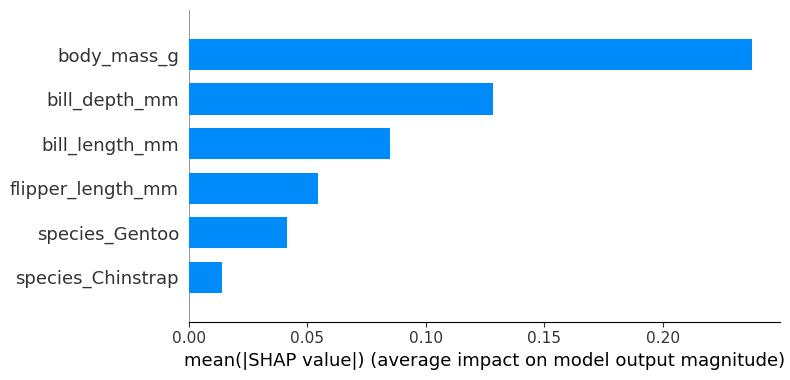
\includegraphics[width=0.6\linewidth]{images/shap-importance.jpg}
	\end{center}
	\caption{SHAP Feature Importance}\label{fig:shapimportance}
\end{figure}

\textbf{SHAP Summary Plot}
\begin{figure}[H]
	\begin{center}
		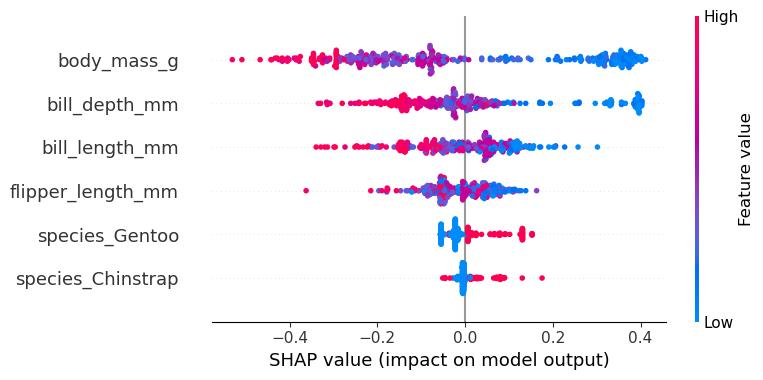
\includegraphics[width=0.6\linewidth]{images/shap-importance-extended.jpg}
	\end{center}
	\caption{SHAP Summary}\label{fig:shap-importance-extended}
\end{figure}
Overlapping points are offset in the y-axis direction, gives a sense of the distribution of Shapley values per features.


\textbf{SHAP Dependence Plot}
\begin{figure}[H]
	\begin{center}
		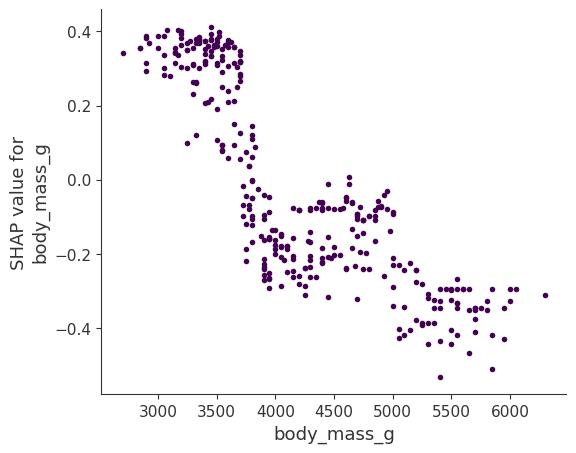
\includegraphics[width=0.6\linewidth]{images/shap-dependence.jpg}
	\end{center}
	\caption{SHAP Dependence Plot}\label{fig:shap-dependence}
\end{figure}
\begin{itemize}
	\item Like PDP/ALE, but shows full distribution, not only average
	\item Variance reveals interactions. (interactions = higher variance)
\end{itemize}
We can plot the interaction values in the dependence plot.

\begin{figure}[H]
	\begin{center}
		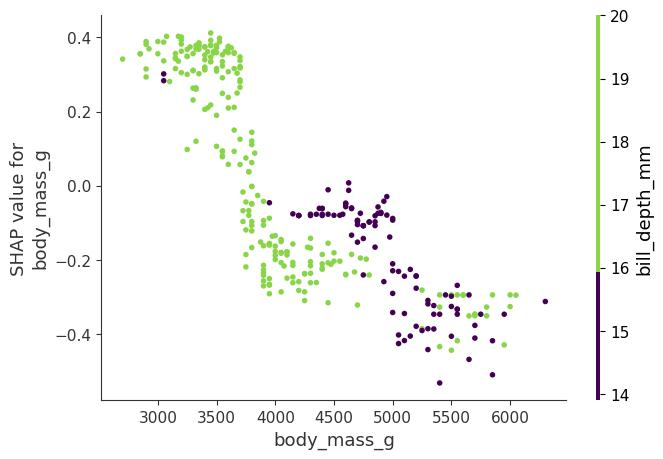
\includegraphics[width=0.6\linewidth]{images/shap-dependence-interaction.jpg}
	\end{center}
	\caption{Plots the dependence plot for one feature and the color signals the interaction with another feature.}\label{fig:dependenceinteractionshap}
\end{figure}

\textbf{Clustering SHAP}
\begin{figure}[H]
	\begin{center}
		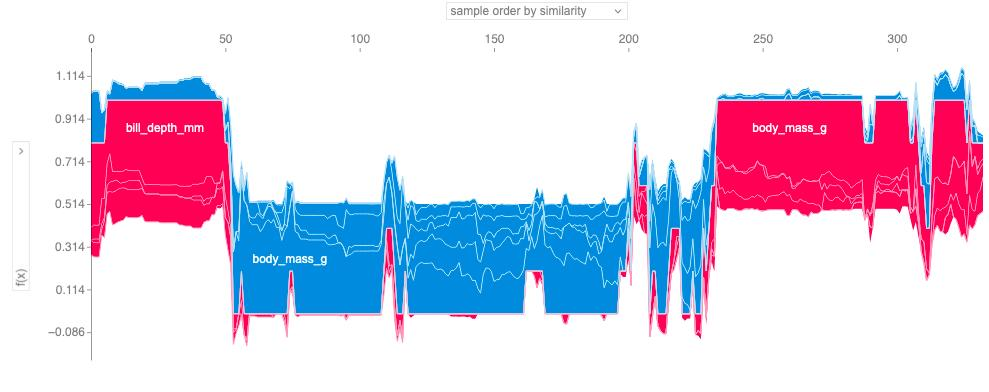
\includegraphics[width=0.8\linewidth]{images/shap-clustering.jpg}
	\end{center}
	\caption{Stacked SHAP explanations clustered by explanation similarity}\label{fig:clusteringshap}
\end{figure}
\begin{itemize}
	\item Force Plots for all instances side by side, clustered by similarity
	\item Identify distinct risk profiles or behavior groups
\end{itemize}


\paragraph{SHAP Notes}
\begin{itemize}
	\item Shapley Advantages
	\item Rich sets of plots
	\item Bridges LIME and Shapley, same additivity as LIME but grounded in Axioms.
	\item KernelSHAP is slow
	\item unrealistic combinations of features when features are dependent (like all permutation based methods)
	\item TreeSHAP uses conditional expectations. Can attribute importance to non-influential correlated features.
	\item Shapley disadvantages.
\end{itemize}

Careful when features are strongly correlated or when you need fast, sparse explanations.
